\chapter{Guide d'onda rettangolari} 

\begin{figure}[h]
    \centering
    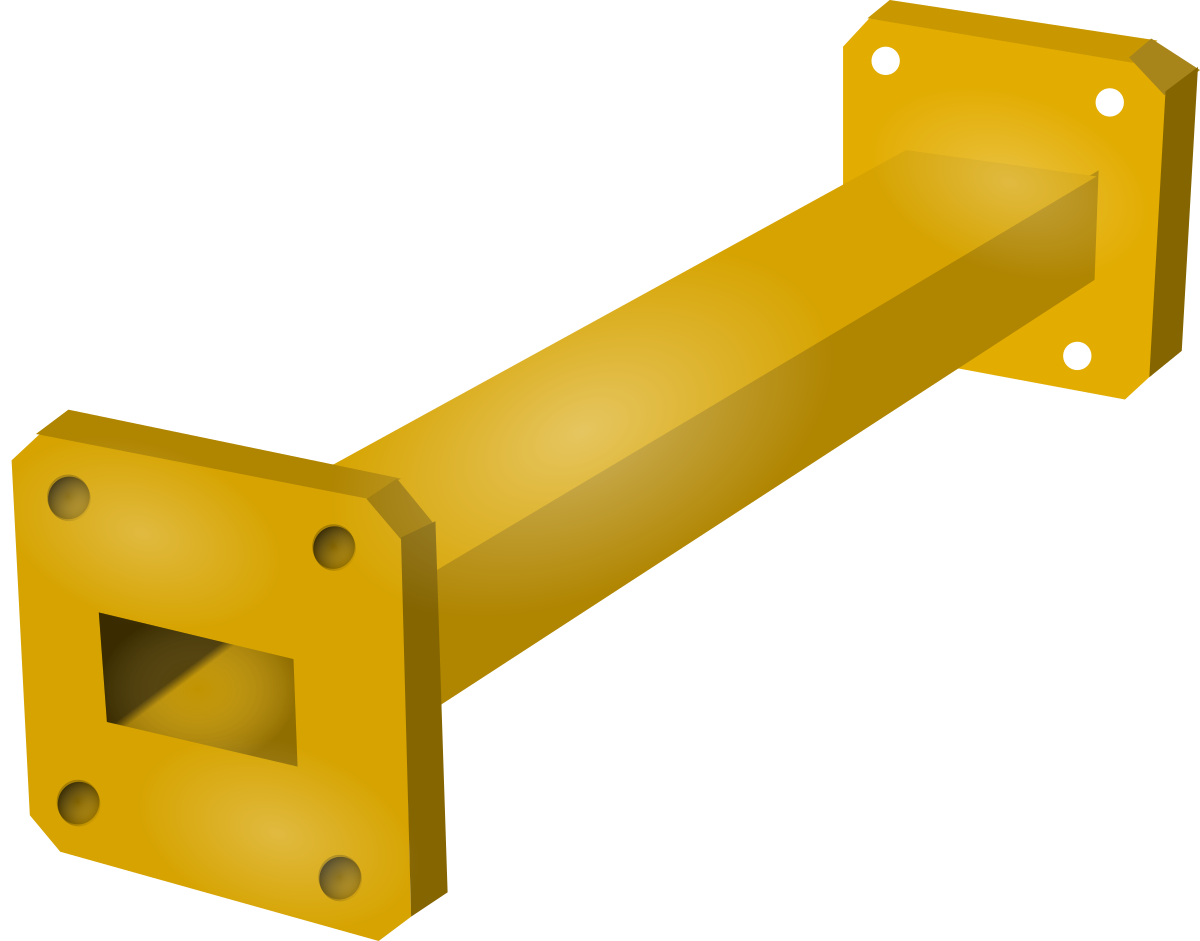
\includegraphics[scale = 0.35]{Waveguide17-with-UBR120-flanges-svg.svg.png}
\end{figure} 

\newpage 

\section{Cosa sono le guide d'onda rettangolari} 

\footnote{FWC - pag 417 \\ 8.7 Rectangular waveguides}

\begin{figure}[h]
    \centering
    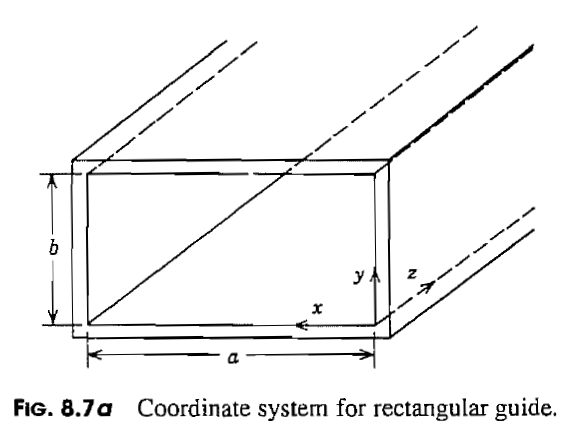
\includegraphics{Coordinate system for rectangular guide.PNG}
\end{figure} 

Le onde rettangolari sono un tipo d'onda in cui la sezione è formata da una regione dielettrica di larghezza 
a e di altezza b che si estende per una lunghezza infinita lungo la direzione z, 
regione dielettrica rivestita da quattro conduttori. \\ 

Non ci possono essere onde TEM perchè la componente lungo z non varia (considerando che nella guida d'onda possono 
esistere onde del tipo $e^{-\jmath \omega t - \gamma z}$ e che quindi variano di $\gamma$ lungo l'asse z). \\ 

Onde TM e TE possono esistere in una guida d'onda rettangolare. 

\newpage 

\section{Onde TM nelle guide d'onda rettangolari} 

\footnote{FWC - pag 418 \\ 8.7 Rectangular waveguides - TM Waves} 

Le onde TM, lungo la componente dell'asse z: 

{
    \Large 
    \begin{equation}
        \begin{cases}
            H_z = 0 \\ 
            E_z \neq 0
        \end{cases}
    \end{equation}
}

Dalle equazioni di Maxwell per le guide d'onda, abbiamo trovato che: 

{
    \Large 
    \begin{equation}
        \nabla_t ^{2} E_z 
        = \frac{\partial ^{2} E_z}{\partial x^{2}} + \frac{\partial ^{2} E_z}{\partial y^{2}}
        = - \kappa_c ^{2} E_z
    \end{equation}
}

dove: 

{
    \Large 
    \begin{equation}
        \kappa_c ^{2} = \kappa_x ^{2} + \kappa_y ^{2}
    \end{equation}
}

Quindi: 

{
    \Large 
    \begin{equation}
        \frac{\partial ^{2} E_z}{\partial x^{2}} + \frac{\partial ^{2} E_z}{\partial y^{2}}
        = - \kappa_c ^{2} E_z
        \Rightarrow 
        \frac{\partial ^{2} E_z}{\partial x^{2}} + \frac{\partial ^{2} E_z}{\partial y^{2}}
        =  - \kappa_x ^{2} - \kappa_y ^{2} E_z
    \end{equation}
}

Utilizzando la separazione delle variabili (x,y) possiamo portare questa 
equazione in un sistema per ogni variabile, cioè: 

{
    \Large
    \begin{equation}
        \begin{cases}
            \frac{\partial ^{2} E_z}{\partial x^{2}} 
            = - \kappa_x ^{2} E_z \\ \\
            \frac{\partial ^{2} E_z}{\partial y^{2}} 
            = - \kappa_y ^{2} E_z  
        \end{cases}
    \end{equation}
}


Il cui risultato è rispettivamente \\ 
per l'asse x: 

{
    \Large 
    \begin{equation}
        A^{'} \sin(\kappa_x x) + B^{'} \cos(\kappa_x x) 
    \end{equation}
}

per l'asse y: 

{
    \Large 
    \begin{equation}
        C^{'} \sin(\kappa_y y) + D^{'} \cos(\kappa_y y) 
    \end{equation}
}

dove $A^{'}$, $B^{'}$, $C^{'}$, $D^{'}$ sono coefficienti reali. \\ 

La separazione delle variabili ci impone di moltiplicare i risultati 
per l'asse x e l'asse y, quindi $E_z$ diventa: 

{
    \Large 
    \begin{equation}
        E_z 
        = 
        (A^{'} \sin(\kappa_x x) + B^{'} \cos(\kappa_x x))  (C^{'} \sin(\kappa_y y) + D^{'} \cos(\kappa_y y))
    \end{equation}
}

Siccome consideriamo le pareti della guida d'onda come perfetti conduttori, 
$E_z = 0$ in: 

{
    \Large 
    \begin{equation}
        \begin{cases}
            x = 0 \\ 
            y= 0
        \end{cases}
    \end{equation}
} 

Allora: 

{
    \Large 
    \begin{equation}
        \begin{cases}
            B^{'}= 0 \\ 
            D^{'}= 0
        \end{cases}
    \end{equation}
} 

Ponendo: 

{
    \Large 
    \begin{equation}
            A^{'}C^{'} = A 
    \end{equation}
} 

e considerando le semplificazioni svolti, $E_z$ diventerà: 

{
    \Large 
    \begin{equation}
        E_z = A \sin(\kappa_x x) \sin(k_y y)
    \end{equation}
}

Per $A \neq 0$, $E_z = 0$ non solo in (0, 0), ma anche in: 

{
    \Large 
    \begin{equation}
        \begin{cases}
            x = a \\ 
            y= b
        \end{cases}
    \end{equation}
}

Essendo il $\sin$ una funzione sinusoidale, possiamo scrivere che
$E_z = 0$ non solo per in (a, b) ma anche in: 

{
    \Large
    \begin{equation}
        \begin{cases}
            \sin(\kappa_x x) = 0 
            \Rightarrow 
            \kappa a = m \pi \\ 
            \sin(\kappa_y y) = 0 
            \Rightarrow 
            \kappa b = n \pi 
        \end{cases}
    \end{equation}
}

dove m e n è un numero intero maggiore di 0. \\ 

Quindi per un'onda $TM_{n m}$, la frequanza di cut-off, cioè 
la frequenza per cui $E_z = 0$ è: 


{
    \Large 
    \begin{equation}
        \begin{split}
            \omega_{c_{m,n}} 
            &= 
            \frac{\kappa_{c_{m,n}}}{\sqrt{\mu \varepsilon}} \\
            &= 
            \frac{1}{\sqrt{\mu \varepsilon}} \sqrt{[(\frac{n \pi}{a}) ^{2} + (\frac{m \pi}{b}) ^{2}]}    
        \end{split}
    \end{equation}
}

Siccome sappiamo che: 

{
    \Large 
    \begin{equation}
        \kappa_c ^{2} = \kappa^{2} - \beta^{2}
    \end{equation}
}

è possibile trovare la costante di fase per le frequenze 

{
    \Large 
    \begin{equation}
        \begin{cases}
            \alpha 
            = 
            \kappa_{c_{m,n}} \sqrt{1 - (\frac{\omega}{\omega_{c_{m,n}}})} 
            \text{  per } 
            \omega < \omega_{c_{m,n}}
            \\ \\
            \beta
            = 
            \kappa \sqrt{1 - (\frac{\omega_{c_{m,n}}}{\omega})} 
            \text{  per } 
            \omega > \omega_{c_{m,n}}
        \end{cases}
    \end{equation}
}

La velocità di fase di gruppo sono rispettivamente: 

{
    \Large
    \begin{equation}
        \begin{cases}
            v_p 
            = 
            \frac{\omega}{\beta} 
            = 
            \frac{v}{\sqrt{1 - (\frac{\omega_{c_{m,n}}}{\omega})}}
            \\ \\
            v_g 
            = 
            \frac{ d \omega}{ d \beta} 
            = 
            v\sqrt{1 - (\frac{\omega_{c_{m,n}}}{\omega})}
        \end{cases}
    \end{equation}
}

\begin{tcolorbox}
    In fisica la velocità di fase è la velocità con cui si propaga la fase di un'onda, sia essa elettromagnetica o meccanica. La velocità di fase può essere visualizzata come la velocità di propagazione di una cresta dell'onda ma non coincide necessariamente con la velocità di propagazione di un segnale (che è più propriamente descritta dalla velocità di gruppo) e quindi può essere più alta della velocità della luce senza violare la relatività ristretta. \\
    \url{https://it.wikipedia.org/wiki/Velocit%C3%A0_di_fase} \\ \\
    La velocità di gruppo di un'onda è la velocità con cui si propagano nello spazio le variazioni nella forma dell'ampiezza dell'onda. \\
    La velocità di gruppo è spesso considerata la velocità a cui l'energia o l'informazione sono trasportate dall'onda. In molti casi questa è una visione accurata, e la velocità di gruppo può essere pensata come la velocità di segnale della forma d'onda. \\
    \url{https://it.wikipedia.org/wiki/Velocit%C3%A0_di_gruppo}
\end{tcolorbox}

\newpage 

\section{Onde TE nelle guide d'onda rettangolari} 

\footnote{FWC - pag 419 \\ 8.7 Rectangular waveguides - TE Waves}

Il procedimento sarà simile al caso precedente delle onde TM, ma cambieranno alcune cose. \\ 

Prima di tutto, nelle onde TE abbiamo che: 

{
    \Large 
    \begin{equation}
        \begin{cases}
            H_z \neq 0 \\ 
            E_z = 0
        \end{cases}
    \end{equation}
}

Inoltre: 
{
    \Large 
    \begin{equation}
        \nabla_t ^{2} H_z 
        = \frac{\partial ^{2} H_z}{\partial x^{2}} + \frac{\partial ^{2} H_z}{\partial y^{2}}
        = - \kappa_c ^{2} H_z
    \end{equation}
}

Facendo lo stesso procedimento della separazione delle variabili del caso TE, abbiamo che: 

{
    \Large 
    \begin{equation}
        H_z 
        = 
        (A^{'} \sin(\kappa_x x) + B^{'} \cos(\kappa_x x)) (C^{'} \sin(\kappa_y y) + D^{'} \cos(\kappa_y y))
    \end{equation}
}

I vari componenti dell'onda saranno: 

{
    \Large
    \begin{equation}
        \begin{split}
            E_x 
            &= 
            -\frac{\jmath \omega \mu}{\kappa_c ^{2}} \frac{\partial H_z}{\partial y}
            \\ \\ \\
            &= 
            - \frac{\jmath \omega \mu \kappa_y}{\kappa_c ^{2}} (A^{'} \sin(\kappa_x x) + B^{'} \cos(\kappa_x x)) (C^{'} \cos(\kappa_y y) - D^{'} \sin(\kappa_y y))
        \end{split}
    \end{equation}
}

{
    \Large
    \begin{equation}
        \begin{split}
            E_y 
            &= 
            \frac{\jmath \omega \mu}{\kappa_c ^{2}} \frac{\partial H_z}{\partial x}
            \\ \\ \\
            &= 
            \frac{\jmath \omega \mu \kappa_x}{\kappa_c ^{2}} (A^{'} \cos(\kappa_x x) - B^{'} \sin(\kappa_x x)) (C^{'} \sin(\kappa_y y) + D^{'} \cos(\kappa_y y))
        \end{split}
    \end{equation}
}

In questo caso, però: 

{
    \Large
    \begin{equation}
        \begin{cases}
            E_x = 0 \text{  per } (x, 0) \Rightarrow C^{'} = 0 \\ 
            E_x = 0 \text{  per } (0, y) \Rightarrow A^{'} = 0 \\ 
        \end{cases}
    \end{equation}
}

Ponendo: 

{
    \Large 
    \begin{equation}
        B = B^{'}D^{'}
    \end{equation}
}

$H_z$ diventa: 

{
    \Large 
    \begin{equation}
        H_z = B \cos(\kappa_x x)\cos(\kappa_y y)
    \end{equation}
}

Per $E_x = 0$ in $y=b$ ,quindi: 

{
    \Large
    \begin{equation}
        \kappa_y b = n \pi
    \end{equation}
}

Per $E_y = 0$ in $x=a$ ,quindi: 

{
    \Large
    \begin{equation}
        \kappa_x a = m \pi
    \end{equation}
}

A differenza delle onde TM, basta solo che sia soddisfatta 
solo una delle due condizioni elencate precedentemente per avere continuità 
dell'onda. \\ 

$\omega_{c_{m,n}}$, $\alpha$, $\beta$, $v_p$ e $v_g$ sono le stesse della $TM_{n, m}$ 

\newpage 
